\ylDisplay
{}% Problem name
{2021}% Year
{mcq}% Round (mcq, theory, experiment)
{6}% Problem nr.
{physics}% Subject (physics, chemistry, biology)
{}% Difficulty (1-3)
{
% Syl:
\ifStatement
A given ray of light suffers deviation close to minimum deviation in an equilateral glass prism $P$. Additional glass prisms $Q$ and $R$ are identical to $P$ are now added close to each other as shown in the figure. If the emerged ray from $P$ enters $Q$ and continues to $R$, then this ray will emerge from $R$ with
\begin{center}
  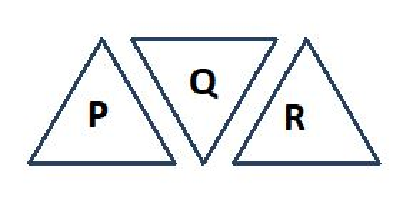
\includegraphics[width=0.3\linewidth]{2021-mcq-06-p}
\end{center}
\fi


\ifOption1
Greater deviation.
\fi


\ifOption2
Same deviation as if P is kept alone.
\fi


\ifOption3
Total internal reflection.
\fi


\ifOption4
No deviation.
\fi


\ifHint

\fi


\ifSolution

\fi


\ifEstStatement
% Problem name:

\fi


\ifEstOption1

\fi


\ifEstOption2

\fi


\ifEstOption3

\fi


\ifEstOption4

\fi


\ifEstHint

\fi


\ifEstSolution

\fi
}
